\section{Multiscale Window Entropies and \texorpdfstring{$2\times 2$}{2x2} Quartet Equivalence}
\label{sec:windows}

Once a permutation reaches the magic ground-state manifold $\ker(\Ltilde_n)$ where $\Hline(S) = 0$, all $2n+2$ global $1\mathrm{D}$ line sums are identical. However, distinct magic squares of the same order exhibit vastly different local $2\mathrm{D}$ spatial organization \cite{dudeney1917amusements,ollerenshaw1998most,cameron2013signatura}. To resolve this internal structure across scales, we introduce sliding $k\times k$ sub-window energies and Shannon entropies, and evaluate them exhaustively across all $880$ Fr\'enicle order-$4$ magic squares and higher-order constructive families.

\subsection{Sliding-Window Shannon Entropy and Constructive Family Scaling}

For any scale $k \in \{1,\dots,n\}$, an $n\times n$ grid contains $M_k = (n-k+1)^2$ interior contiguous $k\times k$ sub-windows $W_{r,c}^{(k)} = \{r,\dots,r+k-1\}\times\{c,\dots,c+k-1\}$ ($1 \le r,c \le n-k+1$). For any exponent $p \in \{1,2,4\}$, define the local $\ell_p^p$ window weight and normalized Shannon window entropy by
\begin{equation}
  w_p\bigl(W_{r,c}^{(k)}\bigr) = \sum_{(i,j)\in W_{r,c}^{(k)}} |Z_{ij}|^p, \qquad
  p_{r,c}^{(k)} = \frac{w_p(W_{r,c}^{(k)})}{\sum_{r',c'} w_p(W_{r',c'}^{(k)})}, \qquad
  \widetilde{H}_p(k) = \frac{-\sum_{r,c} p_{r,c}^{(k)} \log_2 p_{r,c}^{(k)}}{\log_2\bigl((n-k+1)^2\bigr)}.
  \label{eq:window_entropy_def}
\end{equation}
Here $\widetilde{H}_p(k) \in (0,1]$ measures the spatial uniformity of height magnitude across all $k\times k$ sub-windows ($\widetilde{H}_p(k) = 1$ if and only if every $k\times k$ window carries identical $\ell_p^p$ weight).

\begin{figure}[t]
  \centering
  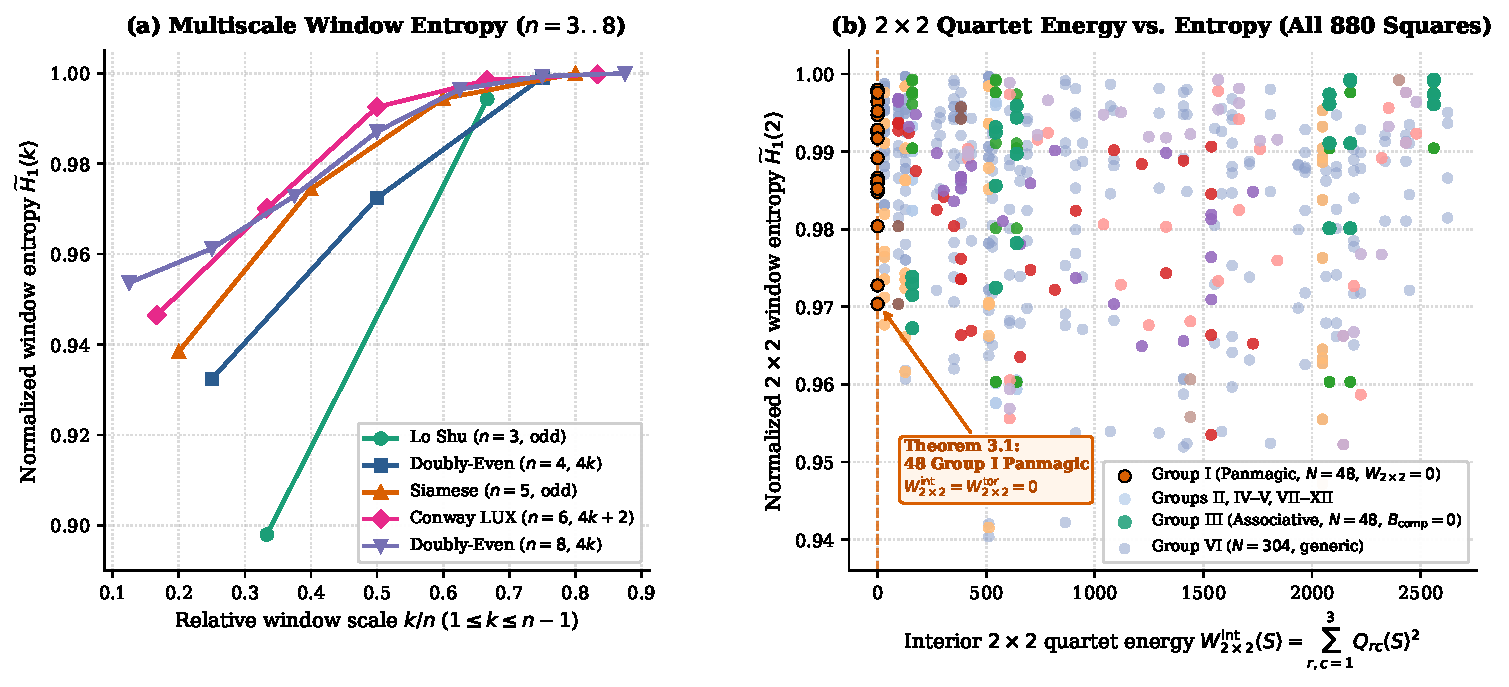
\includegraphics[width=\textwidth]{figures/fig2_window_entropy_880.pdf}
  \caption{\textbf{Multiscale sliding-window Shannon entropy and $2\times 2$ quartet energy census.} \textbf{(a)} Normalized $\ell_1$ window entropy $\widetilde{H}_1(k)$ versus relative scale $k/n$ across five constructive magic-square families ($n=3$ Lo Shu, $n=4,8$ Doubly-Even, $n=5$ Siamese, and $n=6$ Conway LUX). \textbf{(b)} Joint distribution of interior $2\times 2$ quartet residual energy $W_{2\times 2}^{\mathrm{int}}(S)$ and window entropy $\widetilde{H}_1(2)$ across all $880$ Fr\'enicle order-$4$ magic squares partitioned by Dudeney Groups~I--XII, illustrating \Cref{thm:quartet_equivalence}: $W_{2\times 2}^{\mathrm{int}}(S) = 0$ holds if and only if $W_{2\times 2}^{\mathrm{tor}}(S) = 0$, isolating the $48$ panmagic squares of Group~I.}
  \label{fig:window_entropy}
\end{figure}

\Cref{fig:window_entropy}a and \Cref{tab:constructive_families} compare the multiscale entropy profile $\widetilde{H}_p(k)$ across five classical constructive families: odd-order de~La~Loub\`ere (Siamese) squares ($n=3,5$) \cite{loubere1693}, doubly-even $4\times 4$ diagonal-mask squares ($n=4,8$) \cite{andrews1960magic}, and Conway's LUX singly-even construction ($n=6$) \cite{berlekamp2004winning}. At $k=2$, the $3\times 3$ Lo Shu square achieves the highest local uniformity ($\widetilde{H}_1(2) = 0.99435$, $\widetilde{H}_2(2) = 0.99073$), whereas doubly-even mask constructions at $n=4,8$ concentrate extreme values symmetrically in corner and central blocks, lowering $\widetilde{H}_2(2)$ to $0.91498$ ($n=4$) and $0.90598$ ($n=8$). Crucially, while $n=3,4,5,8$ constructions are centrosymmetric ($B_{\mathrm{comp}}=0$ complement breaks and $M_{xyz}=0$), Conway's $n=6$ LUX method breaks all $18/18$ antipodal complement pairs and generates a non-zero mixed octupole moment $M_{xyz} = -132$.

\begin{table}[t]
\centering
\caption{Multiscale window entropy $\widetilde{H}_p(2)$, interior and toroidal $2\times 2$ quartet energies $W_{2\times 2}$, complement breaks $B_{\mathrm{comp}}$, and mixed octupole moment $M_{xyz}$ across constructive magic square families ($n=3\dots 8$).}
\label{tab:constructive_families}
\footnotesize
\setlength{\tabcolsep}{4pt}
\begin{tabular}{@{}llcccccc@{}}
\toprule
Family & Order / Class & $\widetilde{H}_1(2)$ & $\widetilde{H}_2(2)$ & $W_{2\times 2}^{\mathrm{int}}(S)$ & $W_{2\times 2}^{\mathrm{tor}}(S)$ & Breaks $B_{\mathrm{comp}}$ & Octupole $M_{xyz}$ \\
\midrule
Lo Shu (Siamese) & $n=3$ (odd) & $0.99435$ & $0.99073$ & $80$ & $240$ & $0 / 4$ & $0$ \\
Doubly-Even Mask & $n=4$ ($4k$) & $0.97245$ & $0.91498$ & $544$ & $1{,}088$ & $0 / 8$ & $0$ \\
Siamese (de La Loub\`ere) & $n=5$ (odd) & $0.97438$ & $0.94254$ & $16{,}320$ & $25{,}200$ & $0 / 12$ & $0$ \\
Conway LUX Method & $n=6$ ($4k+2$) & $0.97011$ & $0.93161$ & $84{,}640$ & $97{,}440$ & $18 / 18$ & $-132$ \\
Doubly-Even Mask & $n=8$ ($4k$) & $0.96123$ & $0.90598$ & $112{,}320$ & $149{,}760$ & $0 / 32$ & $0$ \\
\bottomrule
\end{tabular}
\end{table}

\subsection{Equivalence of Interior and Toroidal \texorpdfstring{$2\times 2$}{2x2} Quartet Balance at Order 4}

Beyond magnitude entropy, the signed sum of each $2\times 2$ quartet $Q_{r,c}(S) = Z_{r,c} + Z_{r+1,c} + Z_{r,c+1} + Z_{r+1,c+1}$ (with indices taken modulo $n$ in the toroidal case) defines the \emph{interior} and \emph{toroidal $2\times 2$ quartet energies}:
\begin{equation}
  W_{2\times 2}^{\mathrm{int}}(S) = \sum_{r=1}^{n-1}\sum_{c=1}^{n-1} Q_{r,c}(S)^2, \qquad
  W_{2\times 2}^{\mathrm{tor}}(S) = \sum_{r=1}^{n}\sum_{c=1}^{n} Q_{r,c}(S)^2.
  \label{eq:quartet_energies}
\end{equation}
At order $n=4$, $W_{2\times 2}^{\mathrm{int}}$ sums over the $9$ interior $2\times 2$ blocks, whereas $W_{2\times 2}^{\mathrm{tor}}$ includes the $7$ boundary-wrapping blocks. We prove that on the order-$4$ magic manifold, interior quartet balance automatically implies full toroidal quartet balance:

\begin{theorem}[Interior--Toroidal $2\times 2$ Quartet Equivalence]
\label{thm:quartet_equivalence}
Let $S$ be any magic square of order $n=4$. Then its $9$ interior $2\times 2$ blocks have zero centred sum ($W_{2\times 2}^{\mathrm{int}}(S) = 0$) \textbf{if and only if} all $16$ toroidal $2\times 2$ blocks have zero centred sum ($W_{2\times 2}^{\mathrm{tor}}(S) = 0$). Across the $880$ Fr\'enicle magic squares of order $4$, this condition holds on \textbf{exactly the $48$ panmagic (diabolic) squares of Dudeney Group~I} (\Cref{fig:window_entropy}b and \Cref{tab:dudeney_groups}).
\end{theorem}

\begin{proof}
Clearly $W_{2\times 2}^{\mathrm{tor}}(S) = 0 \implies W_{2\times 2}^{\mathrm{int}}(S) = 0$. Conversely, suppose $S$ is an order-$4$ magic square ($\Hline(S) = 0$) with $Q_{r,c}(S) = 0$ for all $1 \le r,c \le 3$. For any horizontally wrapping $2\times 2$ block $Q_{r,4}(S)$ ($1 \le r \le 3$), the sum of rows $r$ and $r+1$ vanishes by magic row balance:
\begin{equation}
  0 = R_{r}(S) + R_{r+1}(S) = Q_{r,1}(S) + Q_{r,3}(S) = Q_{r,2}(S) + Q_{r,4}(S).
  \label{eq:row_pair_partition}
\end{equation}
Since $Q_{r,2}(S) = 0$ by interior balance, \Cref{eq:row_pair_partition} forces $Q_{r,4}(S) = -Q_{r,2}(S) = 0$ for $r \in \{1,2,3\}$. Symmetrically, summing columns $c$ and $c+1$ gives $0 = R_{c_c}(S) + R_{c_{c+1}}(S) = Q_{2,c}(S) + Q_{4,c}(S)$, so $Q_{2,c}(S) = 0 \implies Q_{4,c}(S) = 0$ for $c \in \{1,2,3\}$. Finally, the corner-wrapping quartet $Q_{4,4}(S) = Z_{4,4} + Z_{1,4} + Z_{4,1} + Z_{1,1}$ satisfies $Q_{4,4}(S) = (R_{r_1}(S) + R_{r_4}(S)) - Q_{4,2}(S) = 0 - 0 = 0$. Thus all $16$ toroidal quartets vanish. It is a classical theorem of Fr\'enicle and Dudeney \cite{dudeney1917amusements,ollerenshaw1998most} that a $4\times 4$ magic square has all $2\times 2$ toroidal quartets equal to $2M_4 = 34$ ($Q_{r,c}=0$) if and only if it is panmagic, which characterizes the $48$ squares of Dudeney Group~I.
\end{proof}

\subsection{Centrosymmetric Complement Parity and the Anomalous Octupole Zeros}

In Paper~II \cite{mathewson2026moments} and Paper~III \cite{mathewson2026mechanics}, the mixed third-order moment (octupole) $M_{xyz}(S) = \sum_{i,j=1}^n X_j Y_i Z_{ij}$ governed the asymmetry between static and dynamic axes. To connect $M_{xyz}(S)$ to discrete cell pairing, define the \emph{complement-break count} $B_{\mathrm{comp}}(S)$ as the number of antipodal cell pairs $\{(i,j), (n+1-i, n+1-j)\}$ that fail the associative condition $Z_{ij} + Z_{n+1-i, n+1-j} = 0$ ($s_{ij} + s_{n+1-i, n+1-j} = n^2+1$).

\begin{figure}[t]
  \centering
  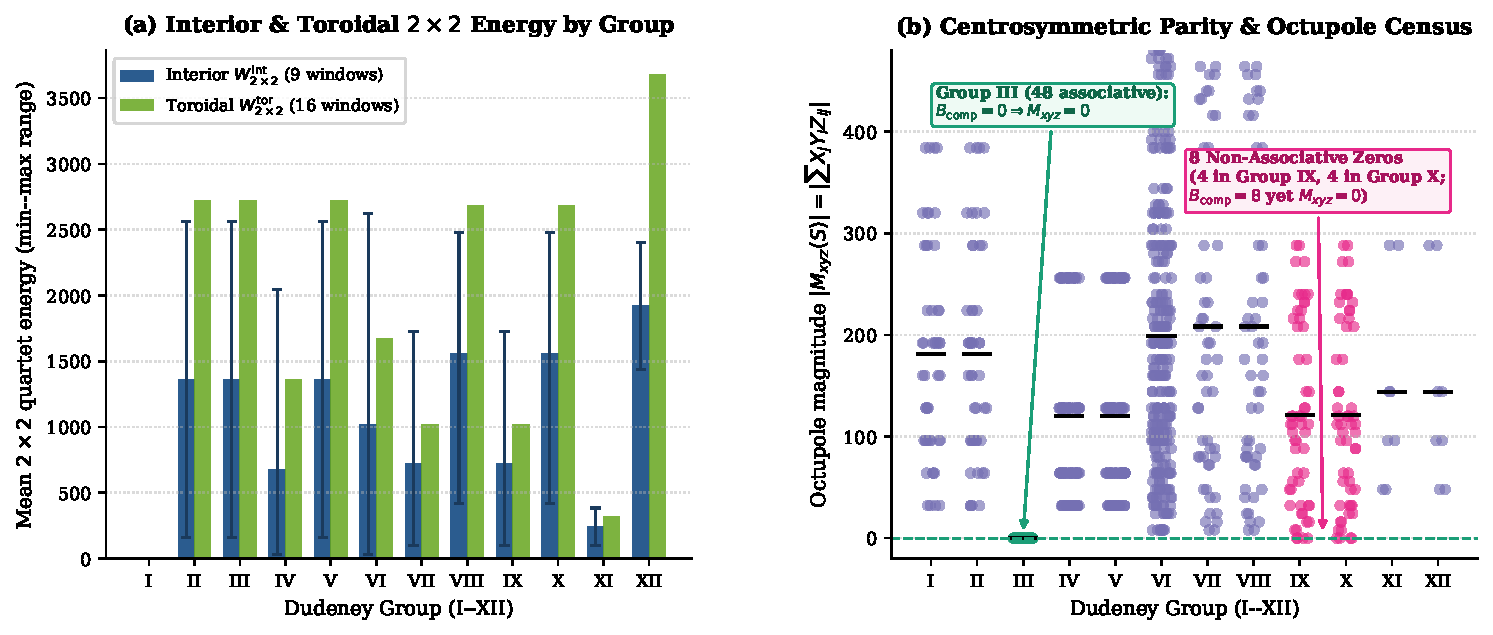
\includegraphics[width=\textwidth]{figures/fig3_octupole_complement.pdf}
  \caption{\textbf{Group-resolved $2\times 2$ quartet energies and mixed octupole census across Dudeney Groups~I--XII.} \textbf{(a)} Mean interior $W_{2\times 2}^{\mathrm{int}}$ ($9$ windows, navy bars with min--max range) and toroidal $W_{2\times 2}^{\mathrm{tor}}$ ($16$ windows, green bars) across the $12$ Dudeney groups. \textbf{(b)} Magnitude of the mixed octupole moment $|M_{xyz}(S)| = |\sum X_j Y_i Z_{ij}|$ across all $880$ squares (\Cref{prop:octupole_census}), highlighting the $48$ associative squares of Group~III ($B_{\mathrm{comp}}=0 \implies M_{xyz}=0$) and the $8$ anomalous non-associative octupole-zero squares in Groups~IX and~X ($B_{\mathrm{comp}}=8$ yet $M_{xyz}=0$).}
  \label{fig:octupole}
\end{figure}

\begin{proposition}[Binary Complement Breaking and Octupole Zero Census]
\label{prop:octupole_census}
Across all $880$ Fr\'enicle magic squares of order $4$:
\begin{enumerate}
  \item \textbf{Binary Complement Breaking:} The complement-break count $B_{\mathrm{comp}}(S) \in \{0,1,\dots,8\}$ takes \textbf{only the two extreme values $\{0, 8\}$}: $B_{\mathrm{comp}}(S) = 0$ on the $48$ associative (symmetric) squares of Dudeney Group~III, and $B_{\mathrm{comp}}(S) = 8$ on all remaining $832$ squares (no order-$4$ magic square has $1 \le B_{\mathrm{comp}}(S) \le 7$).
  \item \textbf{Symmetry-Protected vs.\ Accidental Octupole Zeros:} The mixed octupole moment $M_{xyz}(S) = \sum_{i,j} X_j Y_i Z_{ij}$ vanishes on \textbf{exactly $56$ of the $880$ squares} (\Cref{fig:octupole}b and \Cref{tab:dudeney_groups}):
  \begin{itemize}
    \item All $48$ associative squares of Dudeney Group~III ($B_{\mathrm{comp}}(S) = 0$), where inversion parity $Z_{5-i,5-j} = -Z_{ij}$ combined with $X_{5-j}Y_{5-i} = (-X_j)(-Y_i) = +X_j Y_i$ forces each antipodal pair to cancel: $X_j Y_i (Z_{ij} + Z_{5-i,5-j}) = 0$.
    \item Exactly $8$ non-associative squares ($B_{\mathrm{comp}}(S) = 8$)---$4$ in Dudeney Group~IX and $4$ in Dudeney Group~X---where non-zero antipodal pair sums $Z_{ij} + Z_{5-i,5-j} \ne 0$ cancel algebraically across the $8$ pairs.
  \end{itemize}
\end{enumerate}
\end{proposition}

\begin{table}[t]
\centering
\caption{Complete multiscale window and multipole census across the $12$ Dudeney groups of the $880$ order-$4$ magic squares, verified by \texttt{verify\_paper\_d.py}.}
\label{tab:dudeney_groups}
\resizebox{\textwidth}{!}{%
\begin{tabular}{@{}cccccccc@{}}
\toprule
Dudeney Group & $N_g$ & $B_{\mathrm{comp}}$ & Mean $\widetilde{H}_1(2)$ & Mean $\widetilde{H}_2(2)$ & $W_{2\times 2}^{\mathrm{int}}$ (mean $[\min,\max]$) & $W_{2\times 2}^{\mathrm{tor}}$ (mean) & $|M_{xyz}|$ (mean, $\#=0$) \\
\midrule
I (Panmagic)     & $48$  & $8$ & $0.98722$ & $0.96742$ & $0.0\;[0,0]$         & $0.0$     & $181.3\;(0/48)$ \\
II (Semi-pan.)   & $48$  & $8$ & $0.98148$ & $0.95260$ & $1360.0\;[160,2560]$ & $2720.0$  & $181.3\;(0/48)$ \\
III (Assoc.)     & $48$  & $0$ & $0.98807$ & $0.96789$ & $1360.0\;[160,2560]$ & $2720.0$  & $0.0\;(48/48)$ \\
IV               & $96$  & $8$ & $0.97919$ & $0.94745$ & $680.0\;[32,2048]$   & $1360.0$  & $120.0\;(0/96)$ \\
V                & $96$  & $8$ & $0.98831$ & $0.96951$ & $1360.0\;[160,2560]$ & $2720.0$  & $120.0\;(0/96)$ \\
VI               & $304$ & $8$ & $0.98356$ & $0.95870$ & $1017.7\;[32,2624]$  & $1671.2$  & $199.2\;(0/304)$ \\
VII              & $56$  & $8$ & $0.97874$ & $0.94983$ & $720.6\;[96,1728]$   & $1015.4$  & $208.3\;(0/56)$ \\
VIII             & $56$  & $8$ & $0.98127$ & $0.95081$ & $1554.9\;[416,2480]$ & $2684.0$  & $208.3\;(0/56)$ \\
IX               & $56$  & $8$ & $0.98432$ & $0.95886$ & $720.6\;[96,1728]$   & $1015.4$  & $121.4\;(4/56)$ \\
X                & $56$  & $8$ & $0.98705$ & $0.96844$ & $1554.9\;[416,2480]$ & $2684.0$  & $121.4\;(4/56)$ \\
XI               & $8$   & $8$ & $0.98516$ & $0.96109$ & $240.0\;[96,384]$    & $320.0$   & $144.0\;(0/8)$ \\
XII              & $8$   & $8$ & $0.97871$ & $0.94441$ & $1920.0\;[1440,2400]$& $3680.0$  & $144.0\;(0/8)$ \\
\bottomrule
\end{tabular}%
}
\end{table}

Across all $880$ squares, the global maximum of $2\times 2$ window entropy is achieved by Fr\'enicle square \texttt{\#123} in Group~VI ($\widetilde{H}_1(2) = 0.999669$), while the global minimum occurs at square \texttt{\#599} in Group~VI ($\widetilde{H}_1(2) = 0.940345$). Notice also in \Cref{tab:dudeney_groups} and \Cref{fig:octupole}a that Groups~II, III, and~V share the exact same mean interior quartet energy $\langle W_{2\times 2}^{\mathrm{int}}\rangle = 1{,}360 = \|\mathbf{z}\|^2$ and mean toroidal quartet energy $\langle W_{2\times 2}^{\mathrm{tor}}\rangle = 2{,}720 = 2\|\mathbf{z}\|^2$.
